

%%%%%%%%%%%%%%%%%%%%%%%%%%%%%%%%%%%%%%%%%%%%%%%%%%%%%
%
%
%  	OPTIMIZATION MODELS
%
%
%%%%%%%%%%%%%%%%%%%%%%%%%%%%%%%%%%%%%%%%%%%%%%%%%%%%%




\begin{slide}

\begin{slidesonly}
	\vspace{3cm}
\end{slidesonly}

\begin{center}
\Huge 
\textcolor{LimeGreen}{Optimization Models}
\end{center}

	
\end{slide}




\addcontentsline{toc}{subsection}{Unconstrained Optimization}

\begin{slide}

\question

\begin{problem}[Optimization Problem\footnote{Adapted from ``Mathematical Modelling'' by Meerschaert.}]
A pig weighting 90 kg gains 3 kg per day and cost 45 cents a day to keep. The market price for pigs is 65 cents/kg, but is falling at 1 cent per day. When should the pig be sold?	
\end{problem}

Introduce variables:
\begin{itemize}
	\item $t=$ time at which the pig is sold (in days)
	\item $w=$ weight of the pig (in kg)
	\item $m=$ market price of a pig (in \$/kg)
	\item $C=$ cost of keeping the pig (in \$)
	\item $R=$ revenue from selling the pig (in \$)
	\item $P=$ profit from the sale of the pig (in \$)
\end{itemize}
	

\begin{parts}
	\item Which of these variables depend on $t$? Based on the statement, what do we know about their values?
	\item What is our goal?
	\item Solve the problem.
	\item Answer the question: when should the pig be sold and what is the profit?
\end{parts}

\end{slide}




\addcontentsline{toc}{subsubsection}{Parameter Sensitivity}


\begin{slide}

\SavedDefinitionRender{Sensitivity}

\textbf{Example:} If the time to sell or the profit depends strongly on a parameter, then the model is not very useful.
If the model said to sell at $t=1$ if the daily maintenance cost changed to 46 cents, then the recommendation would be very suspect!

\begin{parts}
\setcounter{partsitem}{4}

	\item Let $(t^\star,P^\star)$ be the optimal values found before. 
	
	What is the sensitivity of $P$ over the parameter $c_d=$ the daily maintenance cost of keeping a pig?
	
	\item Is $S(P^\star,c_d)$ positive/negative? What does that mean? Does that make sense?
	
	\item What is the sensitivity of $P$ over the parameter $m_0=$ the initial market price of a pig (in \$/kg)?

	\item Is $S(P^\star,m_0)$ positive/negative? What does that mean? Does that make sense?

\end{parts}

\end{slide}


\begin{solution}
\begin{slide}
\textbf{Solutions:}
\begin{parts}
	\item 
	\begin{itemize}
 		\item $w(t) = 90 + 3t$
 		\item $m(t) = 0.65-0.01t$
 		\item $C(t) = 0.45t$
 		\item $R(t) = p(t) \cdot w(t)$
 		\item $P(t) = R(t) - C(t)$
 	\end{itemize}
 	\item The goal is to maximize $P(t)$ over $t\geq 0$.
 	\item 	$P(t) = (90+3t)(0.65-0.01t) - 0.45t$ \\
			$\dfrac{dP}{dt} = 3(0.65-0.01t)-0.01(90+3t) - 0.45 = 0$\\
 			$t^\star = 10$ \\	
 			$P^\star(10) = 61.50$
 	\item The pig should be sold on day 10, which will give a profit of \$61.50.

%	\item We have $P = (90+3t)(0.65-0.01t) - c_dt$ and $t^\star = \frac{35}{2} - \frac{50}{3} c_d$.
%
%		We get $P^\star = \frac{25}{3} c_d^2 - \frac{35}{2} c_d + \frac{1083}{16}$ so that
%		\begin{align*}
%		S(P^\star,c_d) 
%			& = \frac{\partial P^\star}{\partial c_d} \frac{c_d}{P^\star} \big|_{c_d=0.45} \\
%			& = \frac{\frac{50}{3} c_d^2 - \frac{35}{2}c_d}{\frac{25}{3} c_d^2 - \frac{35}{2} c_d + \frac{1083}{16}}\big|_{c_d=0.45}
%			= -0.0731707
%		\end{align*}
	\item We have $P = (90+3t)(0.65-0.01t) - c_dt$ so that
		\begin{align*}
		S(P^\star,c_d) 
			& = \frac{\partial P^\star}{\partial c_d} \frac{c_d}{P^\star} \big|_{c_d=0.45} \\
			& = - t^\star \frac{c_d}{P^\star} \big|_{c_d=0.45}
			= -0.0731707
		\end{align*}
		This model is insensitive with respect to the maintenance cost! =)
	\item It is negative, which means that increasing the daily maintenance cost will decrease the profit, which makes sense.
	
	\item We get $S(P^\star,m_0) = 1.26829$, so
%
%		We have $P = (90+3t)(m_0-0.01t) - 0.45t$ and $t^\star = 50m_0-\frac{45}{2}$.
%
%		We get $P^\star = 75 m_0^2 + 22.5 m_0 + 15.1875$ so that
%		\begin{align*}
%		S(P^\star,m_0) 
%			& = \frac{\partial P^\star}{m_0} \frac{m_0}{P^\star} \big|_{m_0=0.65} \\
%			& = \frac{150m_0^2 + 22.5m_0}{75 m_0^2 + 22.5 m_0 + 15.1875}\big|_{m_0=0.65}
%			= 1.26829
%		\end{align*}
		this model is moderately sensitive to the initial price for a pig. =/
		
	\item The sensitivity is positive since increasing the initial price of a pig increases the profit also.
	
\end{parts}


	
\end{slide}

\end{solution}



\begin{slide}

\begin{definition}[Robustness]
How do the results depend on the assumptions?\\

We assumed:
\begin{itemize}
	\item a linear increase in weight of the pig
	\item a linear decrease in the price of the pig	  \\
\end{itemize}
%\hfill\\

What happens if these were nonlinear? The prediction of prices is notoriously uncertain. \\

Prices are often modelled as stochastic processes (like Brownian motion). This would necessitate a different modelling approach.  \\

In particular, we might then want to maximize the expected (average) profit. But if the variance is very large, then the farmer might prefer a lower expected profit if that means lowering the risk (variance). 
The farmer might consider maximizing the expected profit with a constraint on the variance of the profit.
\end{definition}

\end{slide}








\begin{slide}

\question 

\begin{problem}%[Unconstrained Optimization]
	A manufacturer of lawn furniture makes two types of chairs, one with a wood frame and the other with an aluminum frame. The wood frame chair costs \$18 per unit to manufacture and aluminum frame chair costs \$10 per unit to manufacture. The company operates in a market where the number of units that can be sold depends on price. It is estimated that in order to sell $x$ units per day of the wood chair and $y$ units per day of the aluminum chair, the selling price cannot exceed $10 + 31x^{-0.5} + 1.3y^{-0.2}$ dollars per unit for the wood chair and $5 + 15y^{-0.4} + 0.8x^{-0.08}$ dollars per unit for the aluminum chair.
\end{problem}


Let us first investigate the selling price model for \textbf{one type of} chair. %: $P = c_0 + c_1 x^{-a} + c_2 y^{-b}$.

\begin{parts}
	\item As more chairs of both types are sold in the market: $x \to \infty$, what do you expect will happen to their selling price?
	
%	$$ P \to {\rm Cost}$$
	
	\item As chairs become scarce: $x \to 0^+$, what happens to the price?
	
%	$$P \to \infty$$
	
	\item What family of functions satisfies both these conditions?
	
%	$$P = c_0 + c_1 x^{-b}$$
	
\end{parts}
 

%\SavedDefinitionRender{LagrangeMultipliers}
	
\end{slide}


\begin{slide}

\begin{center}
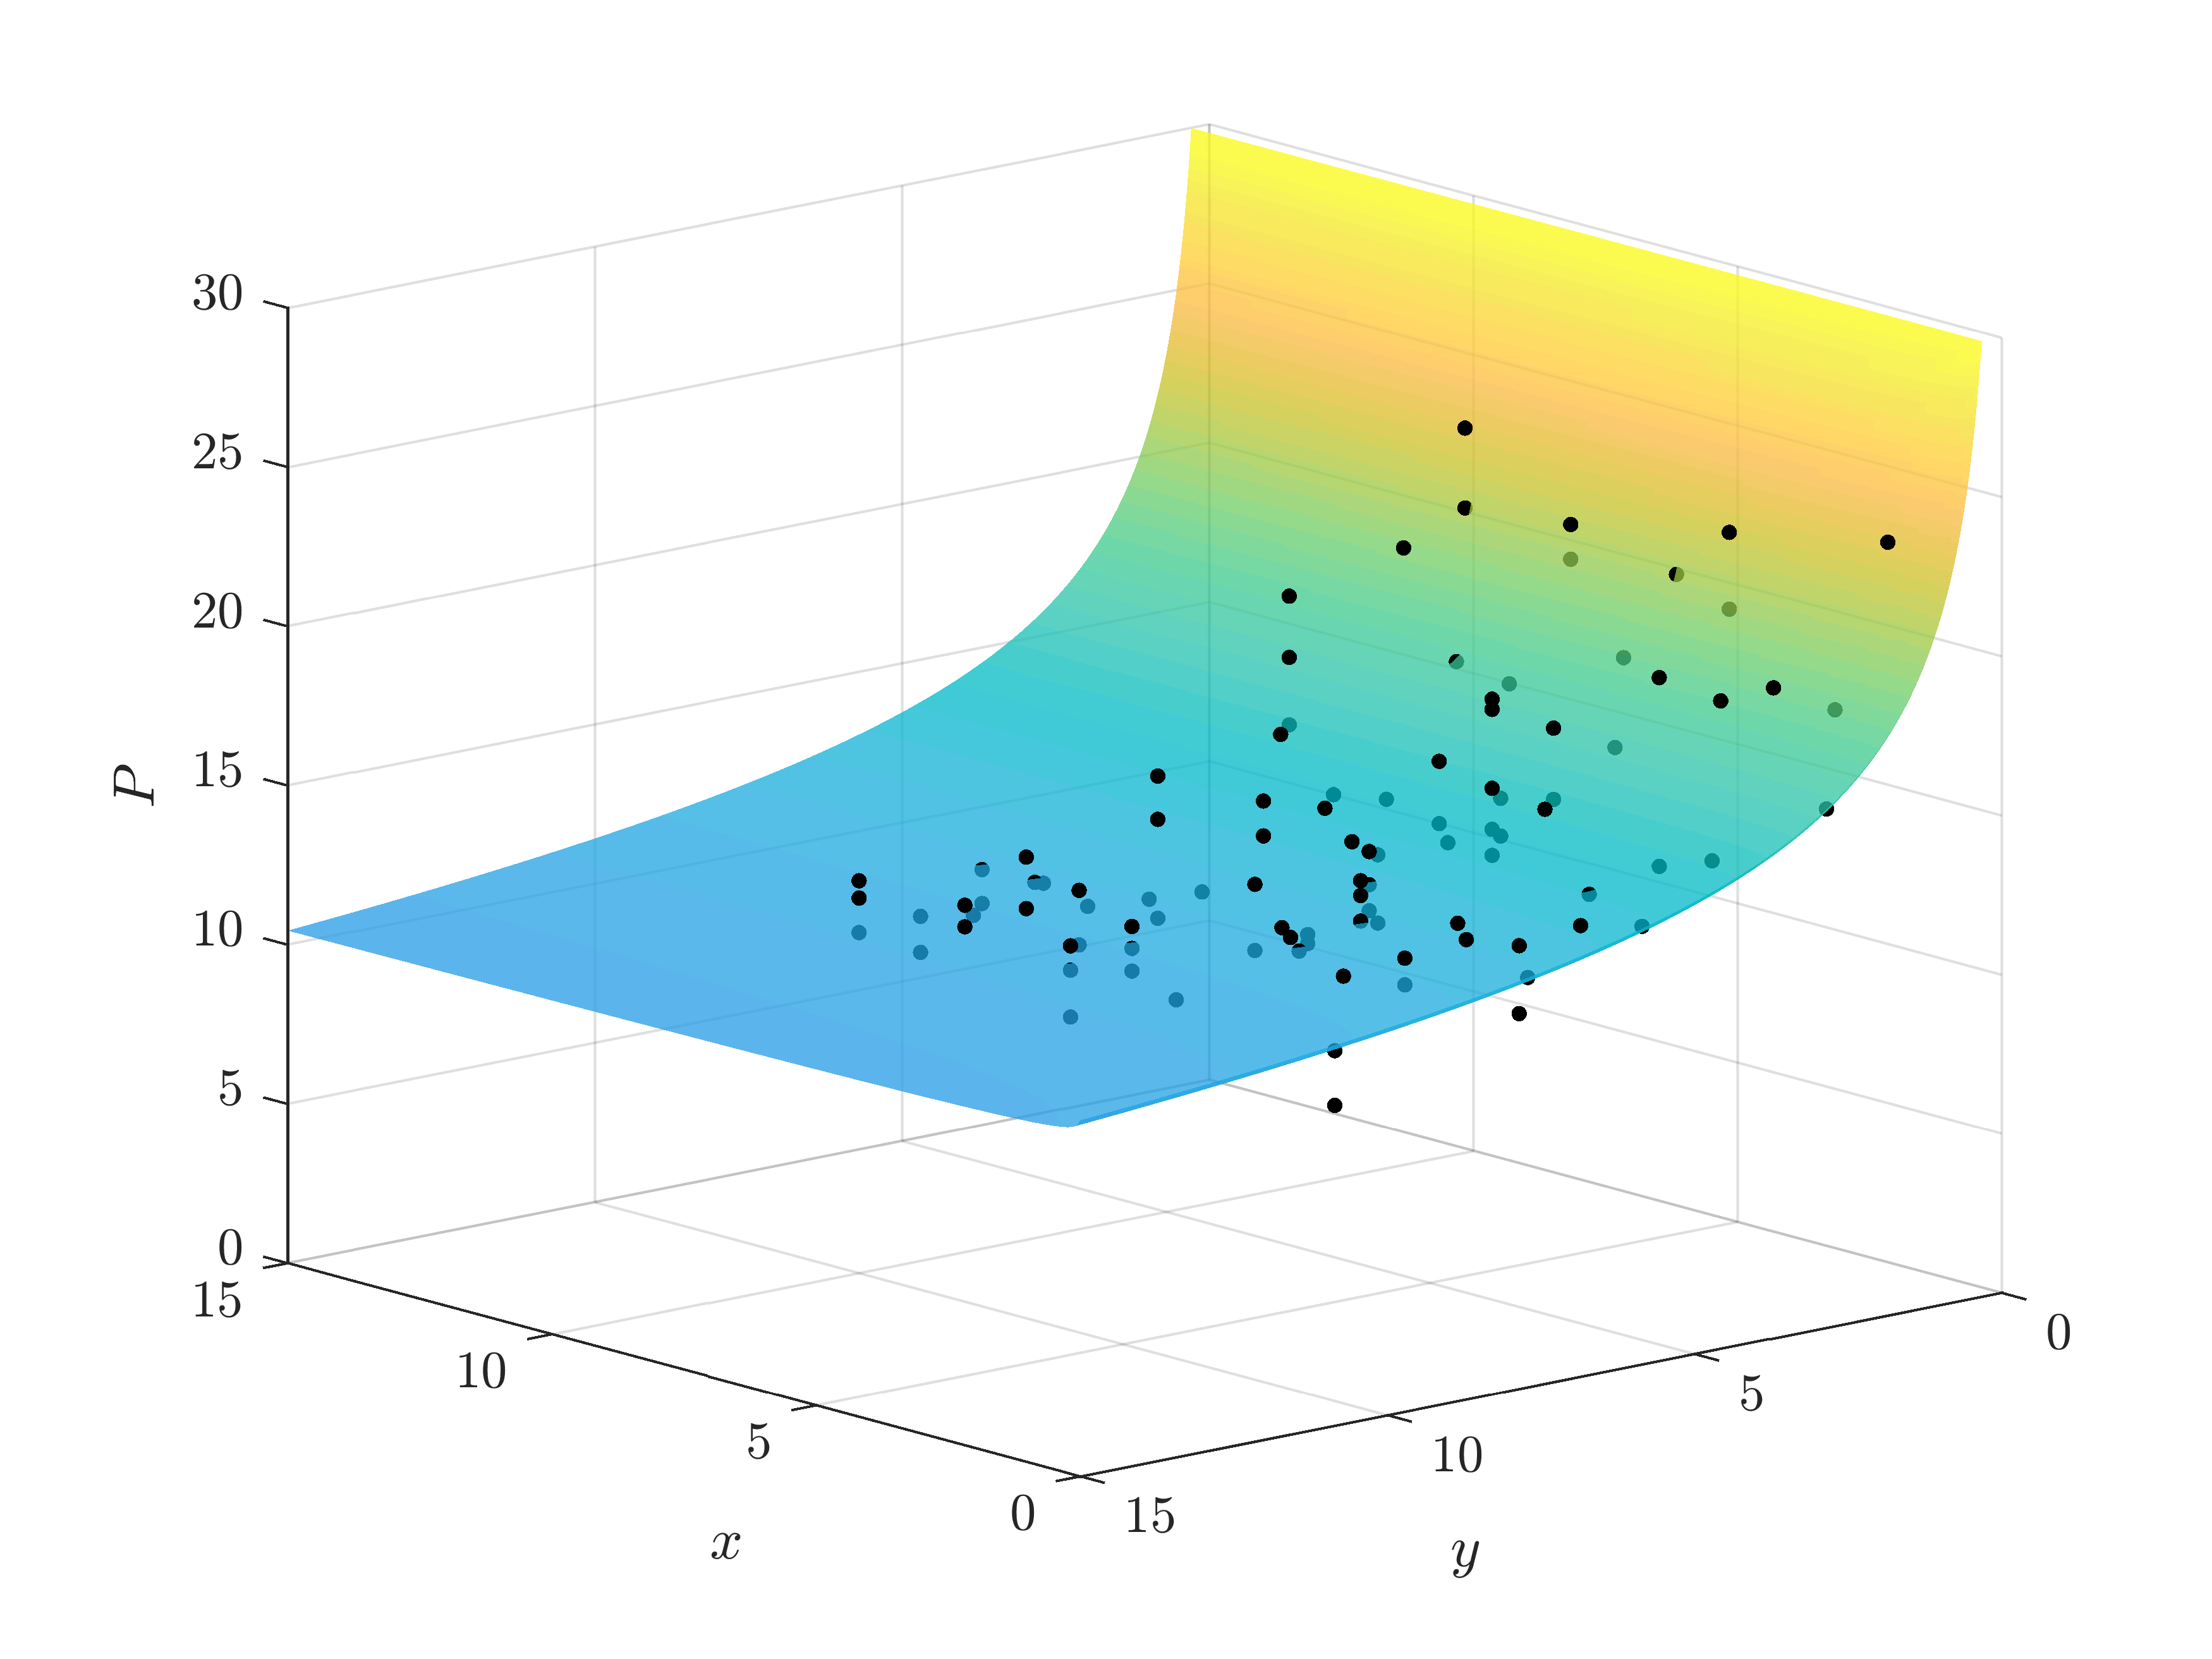
\includegraphics[width=0.6\textwidth]{images/fitprice.png}

Historical prices and fitting surface $p=f(x,y)$.
\end{center}

\end{slide}



\begin{slide}

\question

\begin{problem}%[Unconstrained Optimization]
	A manufacturer of lawn furniture makes two types of chairs, one with a wood frame and the other with an aluminum frame. The wood frame chair costs \$18 per unit to manufacture and aluminum frame chair costs \$10 per unit to manufacture. The company operates in a market where the number of units that can be sold depends on price. It is estimated that in order to sell $x$ units per day of the wood chair and $y$ units per day of the aluminum chair, the selling price cannot exceed $10 + 31x^{-0.5} + 1.3y^{-0.2}$ dollars per unit for the wood chair and $5 + 15y^{-0.4} + 0.8x^{-0.08}$ dollars per unit for the aluminum chair.
\end{problem}


\begin{parts}
	\item We want to maximize the manufacturer's profit. What is the function to maximize?
	\item This is a two-dimensional function, so we need to solve the system
	\begin{align*}
		\frac{\partial f}{\partial x} & = 0 \\[5pt]
		\frac{\partial f}{\partial y} & = 0		
	\end{align*}

	Write down this system.
	\item How can we find the solution?
\end{parts}
	
\end{slide}




\addcontentsline{toc}{subsection}{Newton's Method}


\begin{slide}

\SavedDefinitionRender{Newton1}
\begin{minipage}{0.6\textwidth}
	
\begin{parts}
\setcounter{partsitem}{3}
	\item From the description above, sketch the point $x_1$ on the graph on the right when using Newton's method.
	
	\item What is the formula for $x_1$?
	
\begin{slidesonly}
	\bigskip
\end{slidesonly}
	
	\item Leveraging python.
	\begin{enumerate}
%		\item Go to \url{https://utoronto.syzygy.ca/jupyter}
%		\item Download the file \href{https://raw.githubusercontent.com/bigfatbernie/IBLMathModeling/main/python/chairs_newton.ipynb}{\tt chairs\_newton.ipynb} and import it into the Jupyter Notebook
		\item Clone the file \href{https://utoronto.syzygy.ca/jupyter/user-redirect/git-pull?repo=https://github.com/bigfatbernie/IBLMathModeling&subPath=book/python/chairs_newton.ipynb}{\tt chairs\_newton.ipynb} into your Jupyter Notebook
		\item In the file, introduce the partial derivative functions and an initial guess.
		\item Run the script
	\end{enumerate}
\end{parts}
\end{minipage}
\hfill
	\begin{minipage}{0.35\textwidth}
		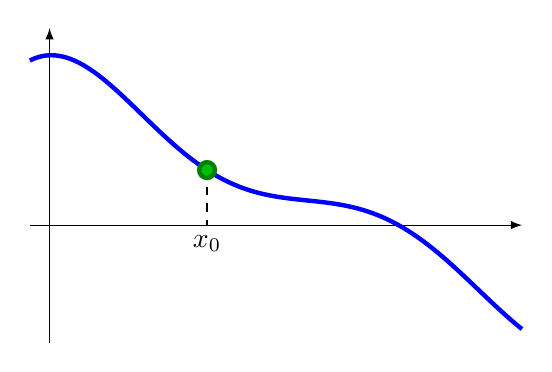
\begin{tikzpicture}%[scale=0.65]
		  \draw[-latex] (0,-1.5) -- (0,2.5);
		    \draw[-latex] (-0.25,0) -- (6,0);
		%    \draw[ultra thick, blue, variable=\x, samples=100,domain=0:8] plot ({\x},{(-1.5*sin(180*(\x-4.5)/pi)*(\x-4.5+0.1(\x-4.5)^3-3*(\x-4.5))/4});
		    \draw[ultra thick, blue, variable=\x, samples=100,domain=-0.25:6] plot ({\x},{(-1.5*sin(180*(\x-4.5)/pi)*(\x-4.5)+0.1*(\x-4.5)^3-3*(\x-4.5)-0.2)/5});
		  \draw[dashed, thick] (2,{(-1.5*sin(180*(2-4.5)/pi)*(2-4.5)+0.1*(2-4.5)^3-3*(2-4.5)-0.2)/5}) -- (2,0) node[below] {$x_0$};
		  \draw[ultra thick, green!50!black, fill=green!75!black] (2,{(-1.5*sin(180*(2-4.5)/pi)*(2-4.5)+0.1*(2-4.5)^3-3*(2-4.5)-0.2)/5}) circle (0.1);
		\end{tikzpicture}
	\end{minipage}

\end{slide}


\begin{slide}

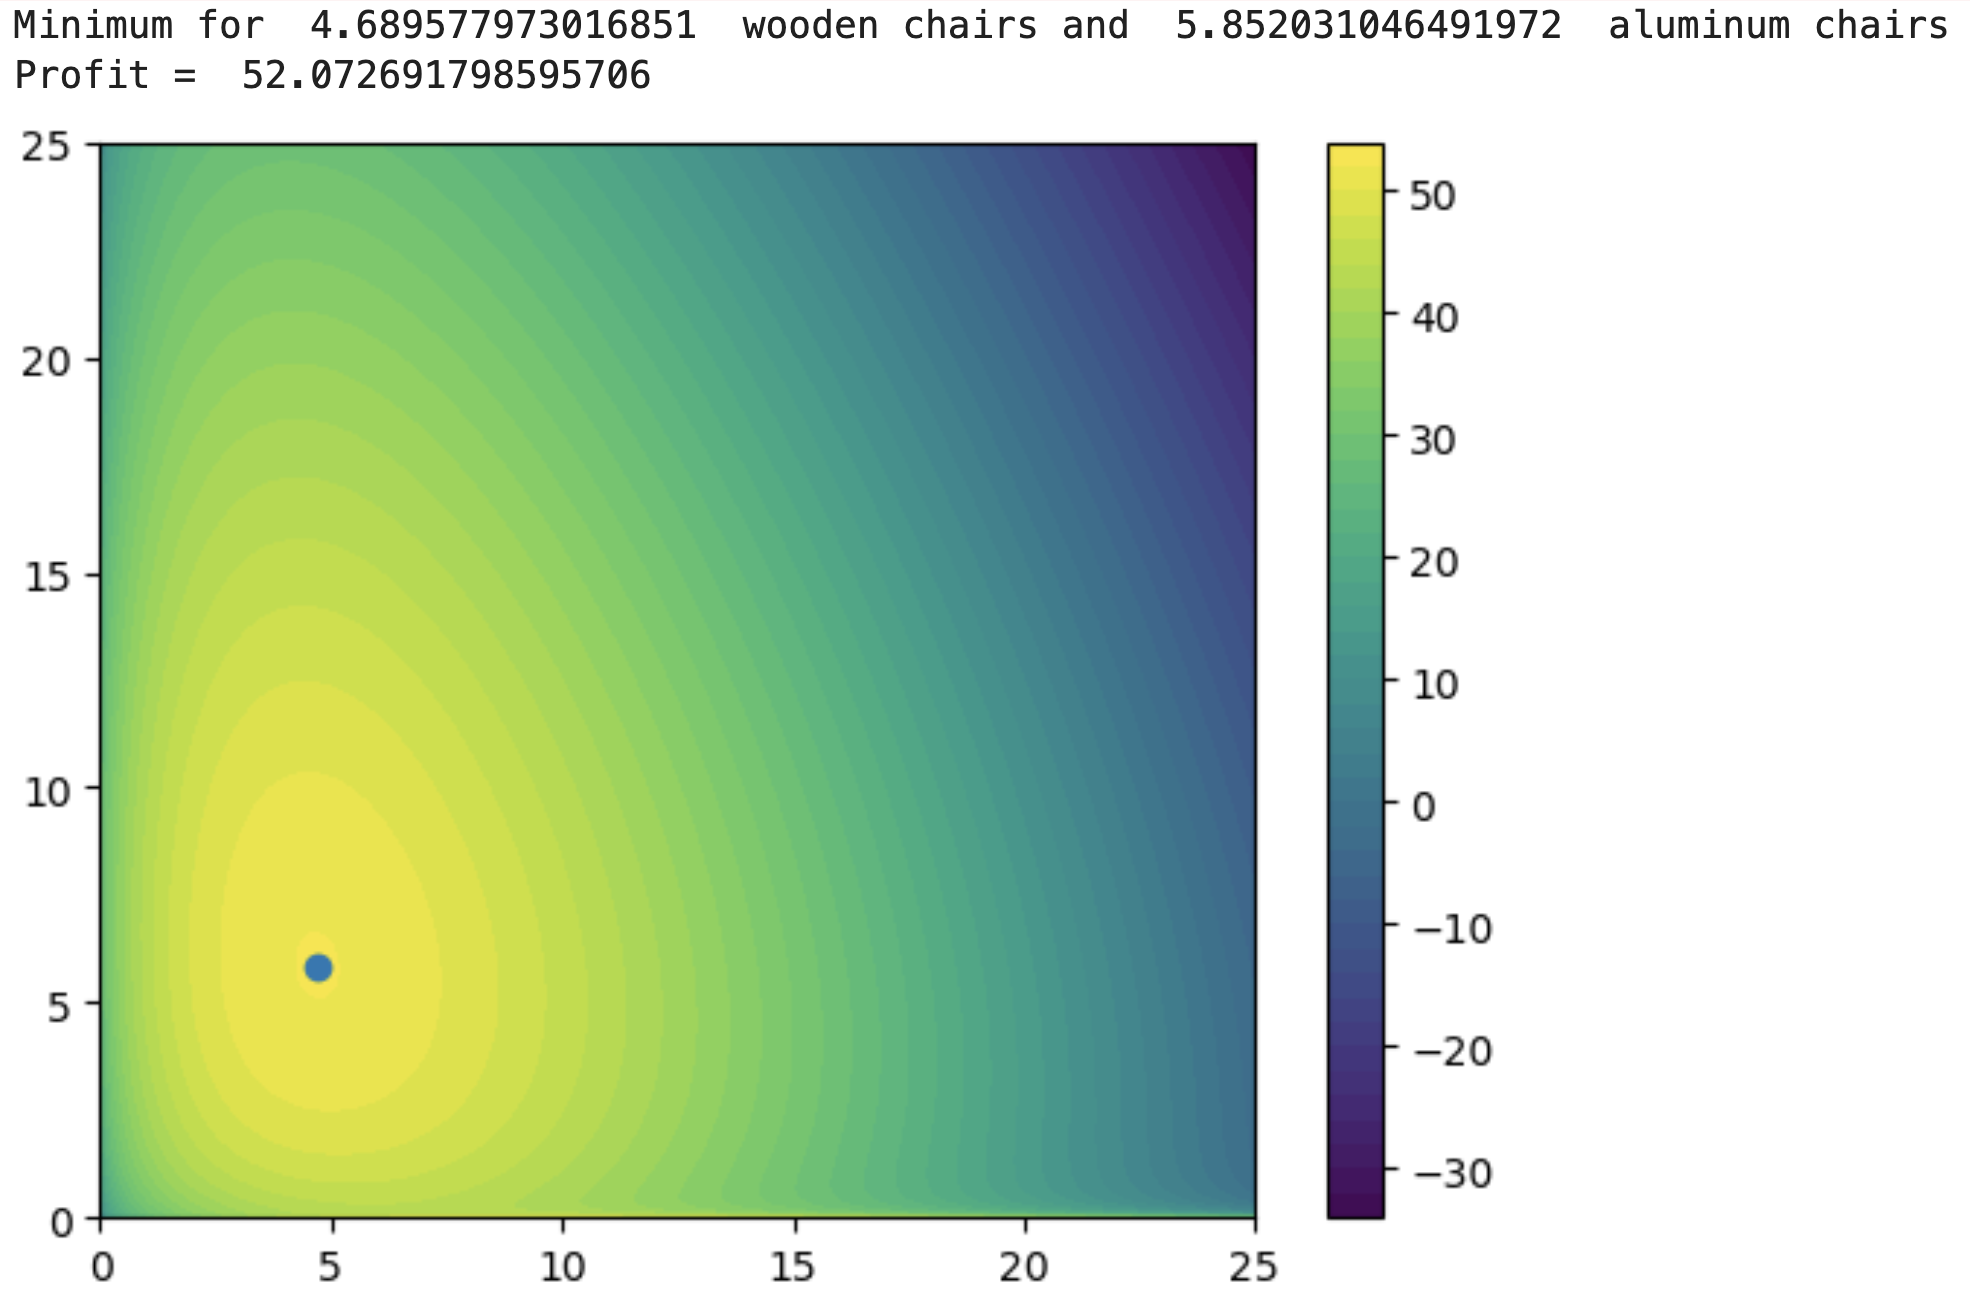
\includegraphics[width=.75\textwidth]{images/chairs-profit.png}
	
\end{slide}

\begin{slide}

\begin{parts}
\setcounter{partsitem}{5}
	\item Leveraging python's minimization tools.
	\begin{enumerate}
%		\item Go to \url{https://utoronto.syzygy.ca/jupyter}
%		\item Download the file \href{https://raw.githubusercontent.com/bigfatbernie/IBLMathModeling/main/python/chairs_fmin.ipynb}{\tt chairs_fmin.ipynb} and import it into Jupyter Notebook
		\item Clone the file \href{https://utoronto.syzygy.ca/jupyter/user-redirect/git-pull?repo=https://github.com/bigfatbernie/IBLMathModeling&subPath=book/python/chairs_fmin.ipynb}{\tt chairs\_fmin.ipynb} into your Jupyter Notebook
		\item In the file, introduce the profit function and an initial guess.
		\item Run the script
	\end{enumerate}
\end{parts}
\end{slide}


\begin{slide}

\question

\begin{problem}%[Unconstrained Optimization]
	A manufacturer of lawn furniture makes two types of chairs, one with a wood frame and the other with an aluminum frame. The wood frame chair costs \$18 per unit to manufacture and aluminum frame chair costs \$10 per unit to manufacture. The company operates in a market where the number of units that can be sold depends on price. It is estimated that in order to sell $x$ units per day of the wood chair and $y$ units per day of the aluminum chair, the selling price cannot exceed $10 + 31x^{-0.5} + 1.3y^{-0.2}$ dollars per unit for the wood chair and $5 + 15y^{-0.4} + 0.8x^{-0.08}$ dollars per unit for the aluminum chair.
\end{problem}


\textbf{Sensitivity}. To compute $p^\star$, you can use \href{https://utoronto.syzygy.ca/jupyter/user-redirect/git-pull?repo=https://github.com/bigfatbernie/IBLMathModeling&subPath=book/python/chairs_sensitivity.ipynb}{\tt chairs_sensitivity.ipynb}.

\begin{parts}
	\item How sensitive is the profit to the parameter $c = 10$ (the production cost of the aluminum chair)
		\[ S(p^\star, c) %= \frac{\partial S}{\partial c} (p^\star,c) \cdot \frac{c}{p^\star(c)} 
			\approx \frac{p^\star(c+h) - p^\star(c)}{h} \cdot \frac{c}{p^\star(c)}?
		\]

	\item How sensitive is the profit to the parameter $b = 0.4$ (the exponent of $y$ in the selling price of the aluminum chair)
		\[ S(p^\star, b) \approx \frac{p^\star(b+h) - p^\star(b)}{h} \cdot \frac{b}{p^\star(b)}?
		\]
\end{parts}

% We already calculated all the terms in these expressions for S except the $p^\star(b+h)$. Those are the only ones we need to calculate.

\begin{solution}
\hspace{-3em}Note that we are using numerical derivatives, since calculating the partial derivatives analytically is usually impossible.	
\end{solution}



\end{slide}






\addcontentsline{toc}{subsection}{Constrained Optimization}


\addcontentsline{toc}{subsubsection}{Lagrange Multipliers}



\begin{slide}

\question

\textbf{Constrained Optimization.} 
How do we solve optimization problems with constraints?

\SavedDefinitionRender{LagrangeMultipliers}


\begin{definition}[Notes:]
\begin{enumerate}
	\item This is a necessary, but not sufficient condition.
	\item To solve the optimization problem, find candidates $x$ that satisfy it, and then pick the best one.
	\begin{itemize}
		\item Points for which $\nabla g_1(x), \ldots, \nabla g_k(x)$ are linearly dependent should also be candidates.
	\end{itemize}
	\item \eqref{LM} $\Leftrightarrow \nabla f(x^\star) \in {\rm span}\Big\{\nabla g_1(x), \ldots, \nabla g_k(x)\Big\}$.
	\item The ``optimal'' values for $\lambda_1, \ldots, \lambda_k$ give important insights on the problem, as we will see -- don't ignore them!
\end{enumerate}
\end{definition}

\end{slide}





\begin{slide}
	
\begin{problem}[Example]
Consider the problem:
\begin{itemize}
	\item Maximize $x+y$ \quad such that $x^2+y^2 = 1$.
\end{itemize}
\end{problem}

\begin{center}
	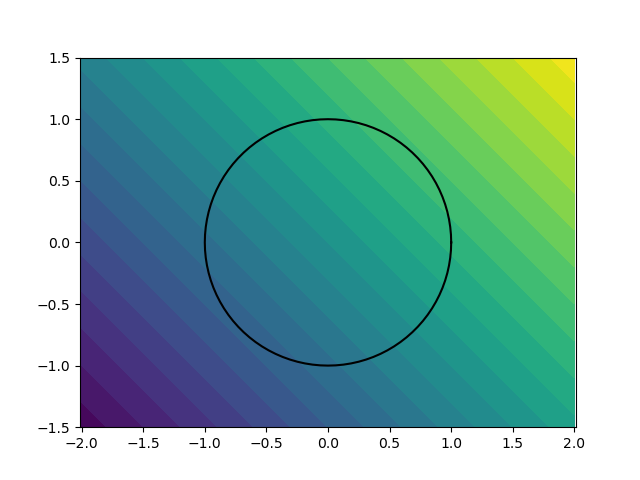
\includegraphics[width=.4\textwidth]{images/LagrangeMultipliers-ex.png}
\end{center}

\begin{parts}
	\item Use Lagrange Multipliers to find the maximum (and the minimum).

	\item If the constraint was $x^2+y^2=c$, then what is:
	\begin{enumerate}
		\item the maximizer point $(x^\star,y^\star)$?
		\item the Lagrange multiplier $\lambda^\star$?
		\item the maximum $f(x^\star,y^\star)$?
	\end{enumerate}
	
	\item Compare $\lambda^\star$ with $\dfrac{\partial f(x^\star,y^\star)}{\partial c}$.
	
	\item Based on this relation, give an interpretation for the Lagrange Multiplier.
	
\end{parts}

\end{slide}


\begin{solution}
\begin{slide}

\begin{parts}
	\item 
	\begin{align*}
		\nabla f & = \mat{1\\1}  
			\quad \text{ and } \quad \nabla g = \mat{2x\\2y} \\
		\\
		\mat{1\\1} & = \lambda \mat{2x \\ 2y} \quad \Leftrightarrow \quad 
			\begin{cases}
				1 & = 2\lambda x \\
				1 & = 2\lambda y \\
				1 & = x^2 + y^2	
			\end{cases}
			\\
		1 & = \frac{1}{2 \lambda^2} \quad \Leftrightarrow\quad 
			\lambda = \pm\frac{1}{\sqrt{2}}\\
		x & = y = \pm \frac{1}{\sqrt{2}}
	\end{align*}
	
	\item $x^\star=y^\star= \frac{\sqrt{c}}{\sqrt{2}}$ \quad and \quad $\lambda^\star = \frac{1}{\sqrt{2c}}$
		 
		 $\max = x^\star+y^\star=\sqrt{2c}$
		
	\item $\dfrac{\partial f(x^\star,y^\star)}{\partial c}
			= \dfrac{\sqrt{2}}{2\sqrt{c}} = \lambda^\star$

	\item This means that if the constraint increased from $1$ to $1 + \Delta = 1.1$, 	then we would expect the maximum to increase by approximately $\Delta \lambda^\star = \frac{\Delta}{\sqrt{2}} \approx 0.07$.
		
		Indeed, $\Delta f = \sqrt{2.2}-\sqrt{2} \approx 0.069$.

\end{parts}
	
\end{slide}	
\end{solution}


%\begin{solution}
%\begin{slide}
%
%We obtain the following equations:
%\begin{align*}
%	\nabla f & = \mat{1\\1} \\	
%	\nabla g & = \mat{2x\\2y} \\
%	\\
%	\mat{1\\1} & = \lambda \mat{2x \\ 2y} \\
%	\\
%	1 & = 2\lambda x \\
%	1 & = 2\lambda y \\
%	1 & = x^2 + y^2 \\
%	\\
%	1 & = \frac{1}{2 \lambda^2} \\
%	\lambda & = \pm\frac{1}{\sqrt{2}}\\
%	x & = y = \pm \frac{1}{\sqrt{2}}
%\end{align*}
%		
%\end{slide}
%\end{solution}









\begin{slide}

\question

\textbf{Define the problem.}

\begin{problem}
The production side of the electrical power grid\footnote{This example is based on \href{https://sces.phys.utk.edu/~moreo/mm08/method_HLi.pdf}{Huijuan Li in `Lagrange Multipliers and their Applications'}.} consists of hundreds or thousands of power plants that vary in fuel sources (coal, nuclear, hydroelectric, solar, wind, stored energy in the batteries of electric vehicles, etc.) and characteristics (age, efficiency, automated, etc.). 

How can the power consumption load be allocated to these plants to minimize cost?
\end{problem}


\textbf{Make Assumptions.}

\begin{itemize}
	\item Each power plant is summarized by a cost curve which tells how much a given load costs. Generally, the cost per unit time per unit load of operating a power plant is a concave function of load as in the figure below: small and large loads are expensive.
	\item For simplicity, we will approximate these quadratics by a linear function with one parameter: the cost per unit time per unit load is $c(x) =ax+1$, so the cost rate function has the form $f(x)=(ax+1)x = ax^2+x$.
	
	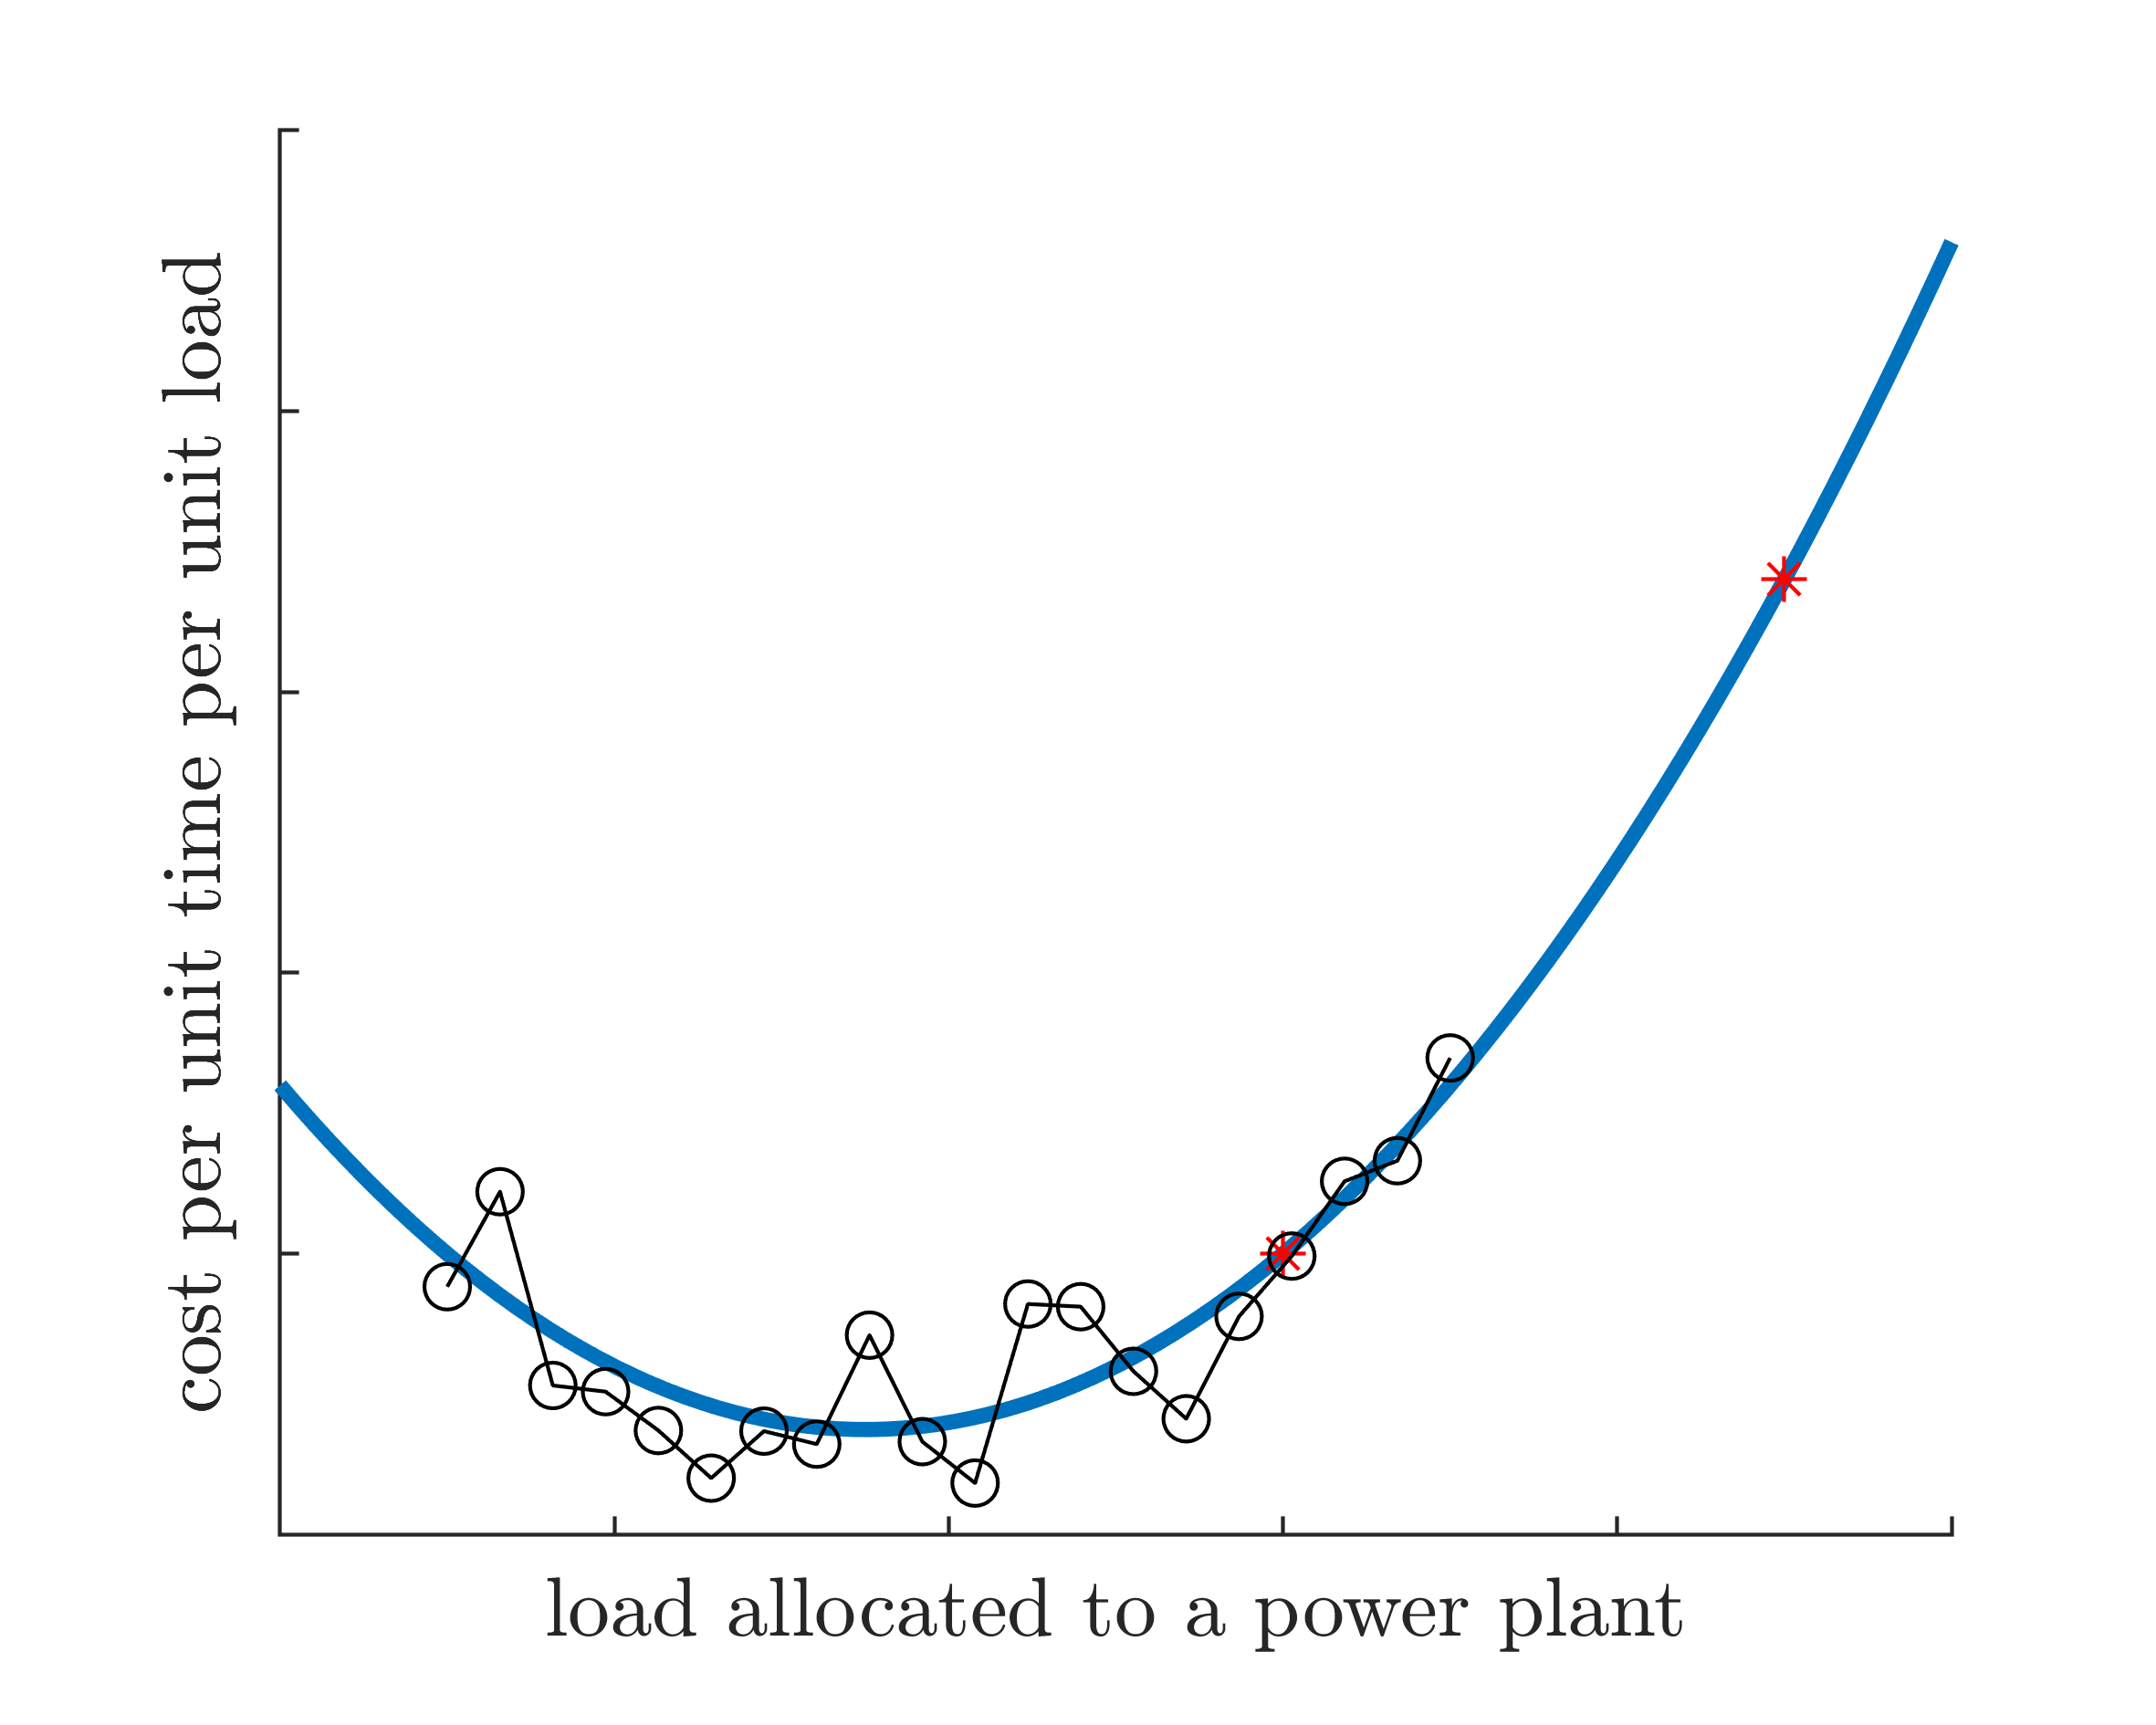
\includegraphics[width=.4\textwidth]{images/concavecost.png} 
	
	\item $N=$ number of power plants
	\item $x_i=$ load assigned to power plant $i$ (in MW)
	\item $X=$ total load (in MW)({In Toronto the average total load is 2500 MW.}).
	\item $C=$ cost rate of power generation (in \$/h)
	\item $f_i(x_i)=$ cost rate function for power plant $i$ (in \$/h)
	

\end{itemize}

	
\end{slide}


\begin{slide}

\textbf{Build a model.}

\begin{parts}
	\item Find an equation relating $X$ and $x_i$.
	\item Find a formula for $C$.
	\item Formulate the problem we want to solve.
	

\begin{slidesonly}
	\bigskip
\end{slidesonly}

\hspace{-2em}
\textbf{Assess the model.}

\hspace{-2em}
	We are going to assume the following:
	\begin{itemize}
		\item Three power plants identified with the parameters:
		\begin{itemize}
			\item $a_1 = 0.0625 $
			\item $a_2 = 0.0125 $
			\item $a_3 = 0.0250 $
		\end{itemize}
		\item The total load is 925 MW
	\end{itemize}


	\item Solve the problem.

\begin{slidesonly}
	\vspace{5cm}
\end{slidesonly}

\hspace{-2em}
\textbf{Report the results.}

	\item What is the interpretation of $\lambda^\star$ the ``optimal'' Lagrange multiplier?
	\item What is the sensitivity of the cost with respect to the parameters $a_i$ and $X$? What does that mean about the model?
		
\end{parts}
	
\end{slide}


\begin{solution}
\begin{slide}

\begin{parts}
\setcounter{partsitem}{2}
	\item 	
		\begin{tabular}[t]{ll}
			Objective: 	& $\displaystyle \min \quad \sum_{i=1}^3 a_i x_i^2 + x_i$ \\
			Constraint: & $\displaystyle \sum_{i=1}^3 x_i = X$
		\end{tabular}

	\item Define:
		\begin{align*}
			C(\vec{x}) & = \sum_{i=1}^3 a_i x_i^2 + x_i \\
			g(\vec{x}) & = \sum_{i=1}^3 x_i = X
		\end{align*}
		
		So we have
		\[
			\nabla C (\vec{x}) 
				= \mat{2a_1 x_1 + 1\\2a_2 x_2 + 1\\2a_3 x_3 + 1} 
				= \lambda	\nabla g (\vec{x}) 
				= \lambda \mat{1\\1\\1}
		\]
		
		Which can be written as
		\[ \matc{2a_1 & 0 & 0 & -1\\0 & 2a_2 & 0 & -1\\0 & 0 & 2a_3 & -1 \\ 1 & 1 & 1 & 0} \mat{x_1\\x_2\\x_3\\\lambda} = \mat{-1\\-1\\-1\\ X}
		\]
		
		And we get the unique solution:
		\begin{itemize}
			\item $x_1 = 112$ MW
			\item $x_2 = 560$ MW
			\item $x_3 = 280$ MW
			\item $\lambda = \$15$ /h/MW (shadow cost)
		\end{itemize}
		
		We used: \href{https://utoronto.syzygy.ca/jupyter/user-redirect/git-pull?repo=https://github.com/bigfatbernie/IBLMathModeling&subPath=book/python/power-plants.ipynb}{\tt power-plants.ipynb}
		
		\item If we reduce the total load ($X$) by 1 MW, it would approximately reduce the total cost of operating the three power plants by \$15/h.
		
		So the operator of the power plants should be willing to pay consumers who pump electricity back to the grid up to \$15/h for each megawatt.

		\item 	\begin{itemize}
			\item $S(C,X) \approx 1.875$
			\item $S(C,a_1) \approx 0.000015$
			\item $S(C,a_2) \approx 0.00017$
			\item $S(C,a_3) \approx 0.00007$
		\end{itemize}


	
\end{parts}
	
\end{slide}
	
\end{solution}


\begin{slide}

\question

\textbf{Robustness.} 

\begin{parts}
	\item The parameter $X$ varies significantly (regularly by over 50\% in a day), so understanding it is very important.

\begin{center}
	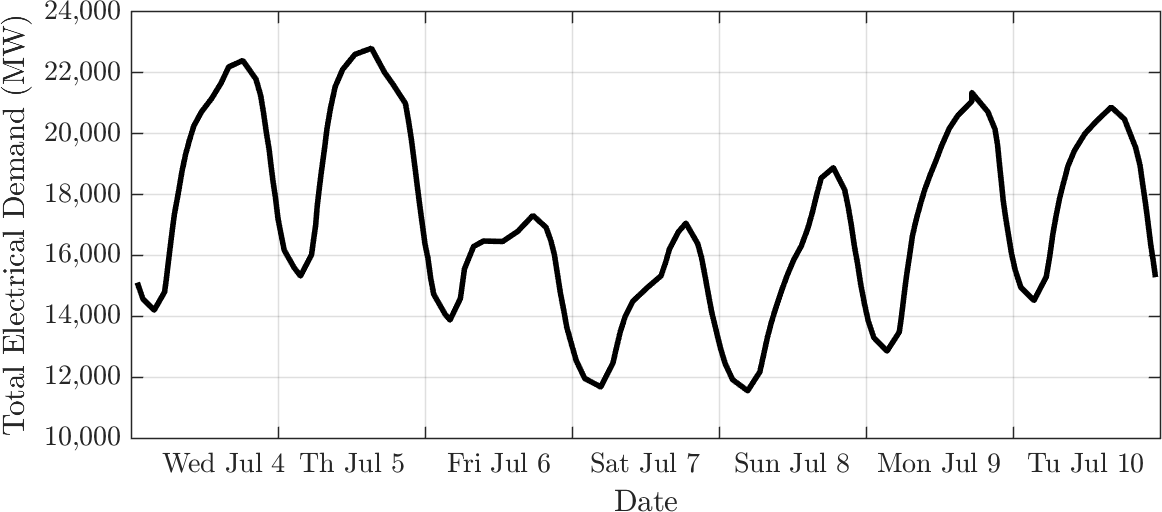
\includegraphics[width=0.4\textwidth]{images/energydemand.png}
\end{center}
	

It is crucial to understand how the optimal cost and loads change with $X$.


	\item Is the quadratic model for $f_i$ good? You can try different functions.
	\item Should there be other constraints on $x_i$? We only imposed $x_i>0$, but we probably should impose upper bounds too.
	\item What about transportation costs? There can be losses of up to 20\% on high-tension transmission lines.
	\item We have a static model, where the power plants operate always at the same load. We might want to consider a dynamic optimization model.
\end{parts}



\end{slide}





\addcontentsline{toc}{subsection}{Linear Programming}


\begin{slide}
\question

\begin{problem}[Linear Programming\footnote{based on a problem from Meerschaert's `Mathematical Modeling'.}]
	A family farm has 1250 hectares\footnote{1 hectare $=1$ ha $=$ 10\,000 m$^2$.}  of land for planting. Possible crops that they could plant are corn, wheat, and oats. There are 400 hectare-m (a volume) of water available for irrigation and 600 hours of labour per week available. The requirements and expected yields are shown below.
	
	
	\begin{center}
	\small
	\begin{tabular}{l|c|c|c}
	%\hline
	& corn & wheat & oats \\ \hline
	irrigation (ha-m / ha) & 1.0 & 0.3 & 0.5 \\ \hline
	labour (person-h / week / ha) & 1.6 & 0.4 & 0.6 \\ \hline
	yield (\$/ha) & 1400 & 420 & 700 \\ %\hline
	\end{tabular}
	\end{center}
	
	We want to maximize the total yield.
\end{problem}

Introduce the following variables:
\begin{itemize}
	\item $x_i= $ hectares planted of $i=1$ corn, $i=2$ wheat, $i=3$ oats
	\item $w=$ the total irrigation used in ha-m
	\item $\ell=$ the total labour used in person-h / week
	\item $a=$ the total area planted in hectares
	\item $y=$ the total yield in \$
\end{itemize}

\begin{parts}
	\item Find expressions for $w, \ell, a, y$
	\item What are the constraints on the variables defined?	
	\item Formulate the optimization problem we want to solve in standard linear programming form:
	\begin{center}
		\begin{tabular}{lc}
		Objective: 		& max \ $\vec{c}^T \vec{x}$ \\
		\multirow{2}{*}{Constraints:} 	& $A \vec{x} \leq \vec{b}$ \\
						& $\vec{x} \geq \vec{0}$
		\end{tabular}
	\end{center}
	\item Use \href{https://utoronto.syzygy.ca/jupyter/user-redirect/git-pull?repo=https://github.com/bigfatbernie/IBLMathModeling&subPath=book/python/farm-linearprog.ipynb}{\tt farm-linearprog.ipynb} to find the solution.

\end{parts}

\end{slide}


\begin{solution}
\begin{slide}
\begin{parts}
	\item
		\begin{itemize}
			\item $w = 1x_1 + 0.3x_2 + 0.5 x_3$
			\item $\ell = 1.6 x_1 + 0.4 x_2 + 0.6 x_3$
			\item $\displaystyle a = \sum_{i=1}^3 x_i$
			\item $y = 1400 x_1 + 420 x_2 + 700 x_3$
		\end{itemize}
		
	\item 
		\begin{itemize}
			\item $x_i \geq 0$
			\item $w \leq 400$
			\item $\ell \leq 600$
			\item $a \leq 1250$
		\end{itemize}
	\item 	\begin{tabular}[t]{lc}
				Objective: 						& max \ $\mat{1400 & 420 & 750} \vec{x}$ \\
				\multirow{2}{*}{Constraints:} 	& $\mat{1 & 0.3 & 0.5\\1.6 & 0.4 & 0.6\\1 & 1 & 1} \vec{x} \leq \mat{400\\600\\1250}$ \\
							& $\vec{x} \geq \vec{0}$
			\end{tabular}
\end{parts}
\end{slide}
\end{solution}

\begin{slide}

We ran the same model with the Wheat Yield ranging from \$400/ha to \$440/ha and obtained the following graphs.
\begin{center}
	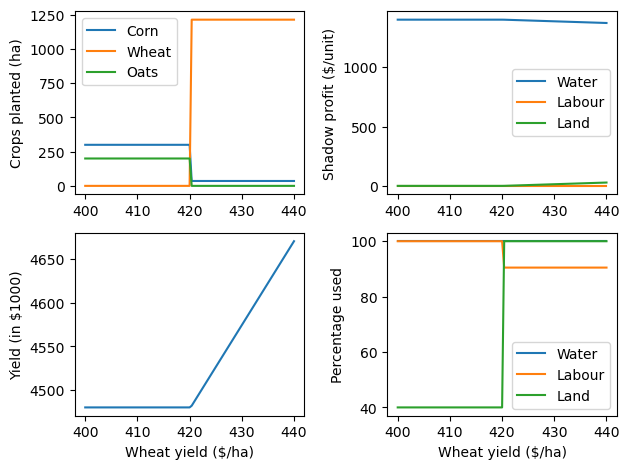
\includegraphics[width=.5\textwidth]{images/farm-linearprog.png}
\end{center}

\begin{parts}
	\setcounter{partsitem}{4}
	\item Interpret the results and the shadow profit ($-$ shadow cost).
\end{parts}
\end{slide}




\begin{slide}
\question

\begin{problem}[Modified farming problem]
We modify the original optimal farming problem to include the notion of plots. The 1250 hectares farm is broken down into 5 plots of 240 hectares each and one 50 hectare plot. For convenience, the farmers want to plot only one crop on each plot. As before, 400 ha-m of water and 600 hours of labour are available. 
The requirements and expected yields are shown below.
	
	\begin{center}
	\small
	\begin{tabular}{l|c|c|c}
	%\hline
	& corn & wheat & oats \\ \hline
	irrigation (ha-m / ha) & 1.0 & 0.3 & 0.5 \\ \hline
	labour (person-h / week / ha) & 1.6 & 0.4 & 0.6 \\ \hline
	yield (\$/ha) & 1400 & 420 & 700 \\ %\hline
	\end{tabular}
	\end{center}
	
	We want to maximize the total yield.
\end{problem}

Introduce the variables:
\begin{itemize}
	\item $x_1, x_2, x_3$ are the number of large plots of corn, wheat, and oats respectively;
	\item $x_4, x_5, x_6$ are the number of small plots of corn, wheat, and oats respectively.
\end{itemize}

\begin{parts}
	\item Set up and solve the problem.
	\item Interpret the results.
\end{parts}

	
\end{slide}


\begin{slide}

\question

\begin{problem}[Ice Cream\footnote{Based on an example from Kamien and Schwartz's `Dynamic Optimization'}]

Suppose a manufacturing company receives an order for $B$ units to be delivered at time $T$, e.g. Sobeys has placed an order for $B = 100$ pallets of Chapman's vanilla ice-cream for a promotion starting in $T = 10$ days.

Chapman's Ice Cream must decide when to produce their tasty product. They don't want to produce it early since they will have to pay to keep it frozen until the order is due. They also do not want to produce it the day before it is due since running the production line fast might have a large cost. %For example, running the machines quickly might have more waste or might produce more and expansive wear-and-tear on the machines.
\end{problem}

Let $x(t)$ be the inventory at time $t$ and suppose that $x(0)=0$ and to fill the order we need $x(T)=B$ (boundary conditions).

\begin{parts}
	\item Let us divide the time interval $[0,T]$ into $N$ ``chunks''. What is the length $\Delta t$ of each?
	\item Let $\Delta x_n$ be the number of units produced during the $n^{\rm th}$ time interval. Find a formula relating $\Delta x_n$ with $x(t)$. Find an equation relating $\Delta x_n$ with $B$.
	\item We need to consider the cost of storing the produced units in inventory: assume that each unit has a cost of $c_2$ per unit time. What is the total inventory cost?
	\item We want to model the fact that running machines faster is more costly. What is a model for the cost of producing $\Delta x_n$ units during a time interval of length $\Delta t$ that quantifies this?
	\item What is the total production cost? 
	\item What is the total cost?
	\item What are the constraints for the variables?
	\item Approximate the solution.
\end{parts}
\end{slide}


\begin{solution}
\begin{slide}

\begin{parts}

\item Let us break the time interval $[0,T]$ into $\Delta t = T/N$ ``chunks'' and consider $t_n=n \Delta t$. We need to decide how many units $\Delta x_n$ to produce at each time interval.

\item We then have:
\begin{itemize}
	\item $x(t_{n+1})) = x(t_n) + \Delta x_n$
	\item $\Delta x_1 + \cdots + \Delta x_N = B$
\end{itemize}

\item We need to consider the cost of storing the produced units in inventory: assume that each unit has a cost of $c_2$ per unit time:
\begin{itemize}
	\item Inventory Cost $\displaystyle = \sum_{n=1}^N \Delta x_n (T-t_n) c_2$
\end{itemize}

\item If the production cost was: $\displaystyle\sum_{n=1}^N c \Delta x_n$, then $c=$ the cost of producing 1 unit in $\Delta t$ time.

If this is constant, then there is no penalty in running the machines faster, so we need to consider $c$ that is not constant and depends on $\Delta x_n$: we make the modelling assumption $c = c_1 \frac{\Delta x_n}{\Delta t}$, so that $c$ is proportional to the rate of production.
We get
\begin{itemize}
	\item Production Cost $\displaystyle = \sum_{n=1}^N  \frac{\Delta x_n^2}{\Delta t} c_1	$
\end{itemize}

\item So the total cost is
\begin{itemize}
	\item Total Cost $\displaystyle = \sum_{n=1}^N \bigg[ \Delta x_n^2 c_1 + \Delta x_n (N-n) c_2 \bigg]$
\end{itemize}

\item The constraints are
\begin{itemize}
	\item $\Delta x_1 + \cdots + \Delta x_N = B$
	\item $\Delta x_n \geq 0$
\end{itemize}

	
\item The solution is here: \href{https://utoronto.syzygy.ca/jupyter/user-redirect/git-pull?repo=https://github.com/bigfatbernie/IBLMathModeling&subPath=book/python/IceCream.ipynb}{\tt IceCream.ipynb}


\end{parts}

\end{slide}
\end{solution}



\addcontentsline{toc}{subsection}{Calculus of Variations}



\begin{slide}
\question \label{q:cv}

In the previous problem, instead of modelling it using \textbf{discrete time}, we can model it using \textbf{continuous time}.

Then, we have the following:
\begin{itemize}
	\item $\frac{dx}{dt}(t) = $ units produced per unit time (at time t)
	\item Inventory cost $\displaystyle= \int_0^T c_2 \frac{dx}{dt}(t) (T-t) \, dt = \int_0^T c_2 x(t) dt$ \hfill (why?)
	\item Production cost $\displaystyle= \int_0^T c_1 \left(\frac{dx}{dt}\right)^2 \, dt$
		\hfill (why?)
\end{itemize}
We can formulate the problem as
\begin{problem}
\begin{tabular}[t]{lc}
	Objective: 						& min \ $\displaystyle\int_0^T c_1 \big(x'(t)\big)^2 + c_2 x(t) ~dt$ \\[10pt]
	\multirow{2}{*}{Constraints:} 	& $x(0)=0$ and $x(T)=B$ \\
				& $x'(t) \geq 0$
\end{tabular}

The goal here is to find a function $x(t)$. This is a problem in \textbf{Calculus of Variations}.
\end{problem}


\end{slide}



\addcontentsline{toc}{subsubsection}{Euler-Lagrange Equation}


\begin{slide}
\question

\begin{problem}[Euler-Lagrange Equation]

We want to find a function $x: [t_0,t_1] \to \R$ that minimizes the functional:
\[ \min \int_{t_0}^{t_1} F \big(t, x(t), x'(t) \big) ~dt \]
and $x(t_0)=x_0$ and $x(t_1)=x_1$.
\end{problem}

When we want to find a minimizer of a function, \textsl{we set the derivative to zero}.



\begin{parts}
	\item The definition of derivative for a real function is
	\[ f'(x) = \lim_{\varepsilon \to 0} \frac{f(x+\varepsilon)-f(x)}{\varepsilon} \]
	
	We only have one direction for $\varepsilon$, so this limit suffices. For a function of multiple variables, we introduced the notion of partial derivative:
	\[ \frac{\partial f}{\partial x_i}(\vec{x}) = \lim_{\varepsilon \to 0} \frac{f(\vec{x}+\varepsilon \vec{e}_i)-f(\vec{x})}{\varepsilon} \]
	
	Our case is similar, but instead of having vectors as inputs, our inputs are functions $x(t)$, so our definition must be adapted to:
	\begin{itemize}
		\item Let $y(t) = x(t) + \varepsilon v(t)$
	\end{itemize}	
	
	What are conditions on $v(t)$ that guarantee that $y(t)$ is an admissible function for the problem formulated in the blue box above?
	
	\item Let $\displaystyle g(\varepsilon) = \int_{t_0}^{t_1} F\big( t, y(t), y'(t) \big) ~dt$. Expand the formula for $g(\varepsilon)$.

	\item Expand $g'(0)$.

	\item Set $g'(0)=0$ and solve.
	
	\textit{Hint: If $\int_a^b f(t) v(t) ~dt=0$ for every function $v(t)$ satisfying $v(a)=v(b)=0$, then $f(t)=0$ for all $t \in (a,b)$.}

\end{parts}
\end{slide}


\begin{slide}
	
\SavedDefinitionRender{EulerLagrange}

\question

We will look back to \textbf{Exercise \ref{q:cv}}.

\begin{parts}
	\item Use the Euler-Lagrange Equation to obtain a Differential equation for $x(t)$.
		
	\item Solve the differential equation with the boundary conditions.
		
	\item We required $x'(t) \geq 0$. Does this solution satisfy this condition?
	
	\item To get a solution that satisfies $x'\geq 0$, we need to consider a solution that doesn't produce any units for a while: 
	\[ x(t) = \begin{cases}
 			0 & \text{ if } t < t_1 \\
 			z(t) & \text{ if } t_1 \leq t \leq T
	 \end{cases}
	 \]
	 
	 What is $t_1$ and what is the function $z(t)$?	
	
	\item If we add a constraint $x'(t) \leq M$, how would that modify the solution? What does this restriction mean in the ice-cream context?
	
\end{parts}
\end{slide}



\begin{solution}
\begin{slide}
\begin{parts}

	\item 
		\begin{align*}
			\frac{\partial F}{\partial x} & = c_2 \\
			\frac{\partial F}{\partial x'} & = c_1 2x'(t) \\
			\frac{d}{dt} \frac{\partial F}{\partial x'} & = 2 c_1 x''(t)
		\end{align*}

		So the Euler-Lagrange equation yields $x''(t) = \frac{c_2}{2c_1}$.
		
	\item 		The general solution of the ODE is: 
			$x(t) = \frac{c_2}{4c_1} t^2 + v_0 t + x_0$
			
		Using the boundary conditions we get:
			\[x(t) = \frac{c_2}{4c_1} t^2 + \frac{4c_1 B-c_2 T^2}{4c_1 T} t\]

	\item 		If $B < \frac{c_2 T^2}{4c_1}$, then $x'$ can be negative at the beginning:
		\begin{align*}
			x'(t) \leq 0 	
				& \Leftrightarrow \frac{c_2}{2c_1} t + \frac{4c_1 B-c_2 T^2}{4c_1 T} \leq 0 \\
				& \Leftrightarrow t \leq \frac{c_2 T^2 - 4c_1 B}{c_2T}	
		\end{align*}
		
		This only happens for small values of $B$. Intuitively, this means that since the order is small, the producer would be better off by selling more of their product to save on inventory (inventory cost becomes negative) and produce the required order later.


	
\end{parts}

\end{slide}	



\begin{slide}
\begin{parts}
	\setcounter{partsitem}{3}

	\item The solution is is decreasing when $c_2 T^2 - 4c_1 B > 0$, so to make sure that this doesn't happen for the new solution, we choose $t_1$ such that $c_2 (T-t_1)^2 - 4c_1 B=0$:
		\[ t_1 = T - \sqrt{ \frac{4c_1 B}{c_2}} \]
	
	The function $z(t)$ is the optimal function $x(t)$ just translated by $t_1$ and with $T \to T-t_1$:
		\[ 
			z(t) = \frac{c_2}{4c_1} (t-t_1)^2 + \frac{4c_1 B-c_2 (T-t_1)^2}{T-t_1} (t-t_1)
		\]

	\url{https://www.desmos.com/calculator/ny2frmc2ov}
	
	\item If $B$ is not too large: $B\leq MT-\frac{c_{2}}{4c_{1}}T^{2}$, then the original solution holds.
		
		If $B$ is too large, then we have too many units to produce in the time provided, so we would need to produce as many as we could ($x'(t)=M$) at the end to be able to complete the order. 
		Before that time, we could produce at the optimal rate.

		\url{https://www.desmos.com/calculator/2rfh1w2a7a}
	
\end{parts}
\end{slide}
\end{solution}




